\documentclass[journal]{IEEEtran}
% correct bad hyphenation here
\hyphenation{op-tical net-works semi-conduc-tor}
\usepackage{graphicx}
%\usepackage[margin=1in]{geometry}
\begin{document}
\title{Page Rank implemented with Hornet}
\author{Giulio~Mazzi (VR406936), Samuele~Germiniani(VR409637)}

% The paper headers
\markboth{}%
{}
\maketitle

% As a general rule, do not put math, special symbols or citations
% in the abstract or keywords.
\begin{abstract}
Discussion of the parallel implementation of the Page Rank algorithm 
in CUDA, using the Hornet framework
\end{abstract}

\section{Introduction}
\IEEEPARstart{T}{his} demo file is intended to serve as a ``starter file''
for IEEE journal papers produced under \LaTeX\ using
IEEEtran.cls version 1.8b and later.
% You must have at least 2 lines in the paragraph with the drop letter
% (should never be an issue)

% needed in second column of first page if using \IEEEpubid
%\IEEEpubidadjcol

\section{Page Rank Algorithm}
PageRank is one of the most known and influential algorithms for computing the
relevance of web pages, and is used by Google, the most successful search
engine on the web. The basic idea of PageRank is that the importance of a web
page depends on the pages that link to it. For instance, we create a web page i
that includes a hyperlink to web page j. If there are a lot pages also link to
j, we then consider j is important on the web. On the hand, if j only has one
in-link, however, this link is from an authoritative web page k (like
www.google.com, www.yahoo.com, or www.bing.com), we also think j is important
because k can transfer its popularity or authority to j.
In general, if a page has k out-links, it will pass on ${\frac{1}{k}}$ of its
importance to each of the pages that it links to.
A picture describing the transition graph can be seen in the following figure\\
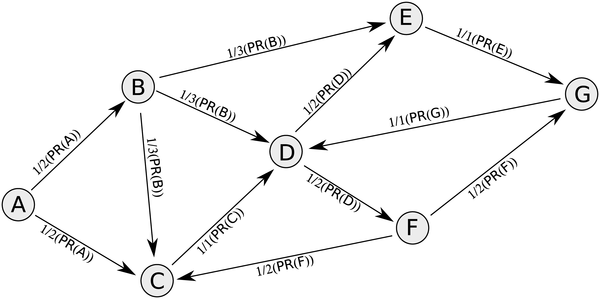
\includegraphics[scale=3.5]{./rappresentazione.png}\\
Suppose that there some pages that do not have any
out-links (we call them dangling nodes), our random surfer will get stuck on
these pages, and the importance received by these pages cannot be propagated.
In the other senario, if our web graph has two disconnected components, the
random surfer that starts from one component has no way to get into the other
component. All pages in other component will receive 0
importance.  Dangling nodes and disconnected components actually are quite
common on the Internet, considering the large scale of the web. In order to
deal with these two problems, a positive constant d between 0 and 1 (typically
0.15) is introduced, which we call the teleport parameter.
A smaller, but positive percentage of the time, the surfer will dump the
current page and choose arbitrarily a different page from the web, and 
teleports” there. The teleport parameter d reflects the probability that the
surfer quits the current page and “teleports” to a new one. Since every page
can be teleported, each page has 1 probability to be chosen.
Page rank can be implemented in many different ways, the one that we use as
reference was the push-based algorithm as seen in \cite{PR}.
We report the pseudo code in table \ref{pseudocode}.\\
The main idea is to compute a residual for every node, based on the ingoing
edges. When the residual is greater than a fixed threshold the
page rank value related to that residual is increased, and so the residual of
the neighbourn of the node must be recomputed. The algorithm uses a queue to
store the node that must be updated.
The sequential implementation of our code implement this tecnique, with the
CPU interface of Hornet.

\begin{table}[]
\centering
\caption{Pseudocode of the sequential algorithm}
\label{pseudocode}
\normalsize
\begin{tabular}{|l|}
\hline
\begin{tabular}[l]{l @{}c@{}}
Push-based PageRank \\
\textbf{Input:} graph G = (V, E), $\alpha$, $\epsilon$  \\
\textbf{Output:} PageRank x \\
1: Initialize $x = (1 \mbox{-} \alpha)e$ \\
2: Initialize r = 0 \\
3:$for$ $ v \in  V do $\\
4:\quad $for$ $ w \in  S_v $ do \\
5: \quad \quad $r_v$  = $r_v  + \frac{1}{|T_w|}$\\
6: \quad end for \\
7:\quad $r_v  = (1  \mbox{-} \alpha )\alpha r_v$ \\
8: end for \\
9:$ for$ $ v \in  V do$\\
10:\quad worklist.push(v) \\
11: end for \\
12: while !worklist.isEmpty do \\
13: \quad $v = worklist.pop()$ \\
14:\quad $x^{new}_v = x_v + r_v$ \\
15:\quad $for$ $ w \in  T_v$ $  do$ \\
16:\quad \quad $r^{old}_w = r_w$ \\
17:\quad \quad $r_w  = r_w  + \frac{r_v \alpha }{|T_v |}$\\
18:\quad \quad if $r_w  \geq \epsilon$  and  $r^{old}_w < \epsilon$  then \\
19:\quad \quad \quad worklist.push(w) \\
20: \quad \quad  end if \\
21:\quad  end for \\
22:\quad $r_v  = 0$ \\
23: end while \\
24:$ x = \frac{x}{\parallel x \parallel _1}$\\
\end{tabular} \\ \hline
\end{tabular}
\end{table}
\section{Parallel implementation} 
\begin{table}[]
\centering
\caption{Pseudocode of the paralle algorithm}
\label{parallel}
\normalsize
\begin{tabular}{|l|}
\hline
\begin{tabular}[l]{l @{}c@{}}
$InitValue()$\\
$bool over\_residual = true$\\
$while ( over\_residual) \{$\\
\quad $updatePageRank(actualResidual) $\\
\quad $newResidual = propagatePageRank(actualResidua)$\\
\quad $actualResidual = moveResidual(newResidual)$\\
\quad $over\_residual = computeThreshold(actualResidual)$\\
\}\\
$normalizePageRank()$
\end{tabular} \\ \hline
\end{tabular}
\end{table}

For the parallel algorithm we use the Hornet framework. Hornet provides
usefull and efficent primivites for graph computation on GPUs.
We start with an overview of our code, and later focus on the ${run}$ function
that implement the core of the algorithm.
Our code has some methods for initilizing the graph and the required data
structure (using the class constructor), and also for setting the parameter
defining the behaviourus of the algorithm (teleport parameter and threshold,
using the ${set\_parameters}$ method).
The algorithm also implements a sequential version of page rank (
${evaluate\_sequential\_algorithm}$, that uses the same graph set in the constructor)
and a method (${validate}$) that compare the sequential and the parallel
results of the algorithms, usefull for testing.
We also provide a testing main, that takes a graph from the standard input
and runs the algorithm on it, reporting a summary of the result.\\

InitValue(), as the name suggests it initialize all the data structure.
The algorithm keep cycling until the sum of the residual are inferior of the
threshold. \\

The algorithm use two vector for storing the residual, one ($actualResidual$)
contains the residual that should be added to the page rank final value,
and $newResidual$ that is the new residual computated after the update of
the page rank.\\
At the beginning of the cycle the redidual previously calculated are moved
to the actual page\_rank value, after that a new residual must be computed,
so every node propagates its $actualResidual$ to all the neighbourns. This is
the most expensive step, as it uses an atomic operation for the sum.
after that the newResidual computetation is terminated and this new residual
becomes the actual residual.\\
In the end, we check if the total sum of the residual is below the
threshold, if so the computation is terminated, otherwise the loop restarts.
After the loop, the page rank must be normalized, with a reduce function we
calculate the total sum of the page rank and we divide all the elements by
this value, so the total sum becomes 1.\\
All the previously mentioned steps, are implemented in a clear a concise
way using $forAllVertices$ and $forAllEdges$ functions, which take the graph,
an operator describing the computation step and some required data like the
residual vector.\\
Lastly we underline the fact that our initial implementation use a queue
like the sequential step, but we realized that that result in worse performance
compared to computing all the node at every iteration step, because the
overhead required to mantain a shared queue overcomes the benefit of reducing
the node that must be recomputed.


\section{Experimental Results} 
\subsubsection{Testing Environment}
We tested our implementation on a AMD Phenom(tm) II X6 1055T with 8gb RAM and 
a GeForce GTX 780.
We compare the performances of our algorithm, a sequential implementation and
another GPU implementation that relied on the Gunrock framework.
\subsubsection{dataset}
We selected some real world graphs with different features such as
nodes number, edges number and average degree.
Must be noted that we removed all the self loop from the graph, because a self
loop in page rank doesn't have much sense, as it makes no sense, for a node,
to give influence to itself.
A complete description of the graphs can be found in table \ref{graph}.
We set 0.001 as threshold for the algorithm and 0.85 as the teleport parameter.

\begin{table}[h]
\centering
\setlength\tabcolsep{5pt}
\caption{Graph Features}
\label{graph}
\begin{tabular}{|c|r|r|c|c|}
\hline
\multicolumn{1}{|c|}{\bfseries Graph Name} & 
\multicolumn{1}{|c|}{\bfseries Nodes} & 
\multicolumn{1}{|c|}{\bfseries Edges} & 
    \multicolumn{1}{|p{0.8cm}|}{\centering \bfseries AVG\\ Degree} & 
\multicolumn{1}{|c|}{\bfseries File size} \\
\hline
belgium\_osm\_nsl.mtx*       &  1.441.295  & 3.099.940   & 2,1        & 22M       \\
cit-Patents\_nsl.mtx*        &  3.774.768  & 16.518.947  & 4,3        & 250M      \\
delaunay\_n21\_nsl.mtx*      &  2.097.152  & 12.582.816  & 6          & 90M       \\
delaunay\_n23\_nsl.mtx*      &  8.388.608  & 50.331.568  & 6          & 378M      \\
delaunay\_n24\_nsl.mtx*      &  16.777.216 & 100.663.202 & 6          & 801M      \\
great-britain\_osm\_nsl.mtx* &  7.733.822  & 16.313.034  & 2,1        & 2123M     \\
hollywood-2009\_nsl.mtx*     &  1.139.905  & 112.751.422 & 98,9       & 757M      \\
italy\_osm\_nsl.mtx*         &  6.686.493  & 14.027.956  & 2,1        & 105M      \\
kron\_g500-logn21\_nsl.mtx*  &  2.097.152  & 182.081.864 & 86,8       & 1.5G      \\
ljournal-2008\_nsl.mtx*      &  5.363.260  & 77.991.514  & 14,5       & 1.2G      \\
rgg\_n\_2\_23\_s0\_nsl.mtx*  &  8.388.608  & 127.002.786 & 15,1       & 953M      \\
roadNet-CA\_nsl.mtx*         &  1.971.281  & 5.533.214   & 2,8        & 40M       \\
road\_usa\_nsl.mtx*          &  23.947.347 & 57.708.624  & 2,4        & 470M      \\
soc-LiveJournal1\_nsl.mtx*   &  4.847.571  & 68.475.391  & 14,1       & 958M      \\
wb-edu\_nsl.mtx*             &  9.845.725  & 55.311.626  & 5,6        & 834M      \\
webbase-1M\_nsl.mtx*         &  1.000.005  & 2.105.531   & 2,1        & 52M       \\
\hline
\end{tabular}
\end{table}

\subsubsection{results}
All the experimental results are shown in table \ref{experiments}.
The results make clear that the parallel implementation can grant meaningfull
speed-up over the sequential implementation. The speed-up isn't fixed but
depends on the graph feature.
The more interesting speed-up is related to Gunrock, Hornet performs better
in nearly all the graph with a speed-up around 5x, except for some graphs in
which the permormance are similar, or show a realy high speed-up (more than
20x).
We have some theories regarding the speed-up, or lack off. First, we notice
that an high average degree result in a realy similar execution time.
This is probably related to the fact that both the algorithm use an ${atomicAdd}$
instruction to calculate the new page\_rank, so the overhead of this function
reduces the advantage of Hornet over Gunrock.
Second, we notice that when the speed up is realy high the number of iteration
of the two algorithm are strongly different. That probably due to better 
implemetation choices in our algorithm w.r.t. the Gunrock one.

\begin{table}[]
\centering
\setlength\tabcolsep{1.5pt}
\caption{Experimental results}
\label{experiments}
\begin{tabular}{|c|c|c|c|c|c|c|c|}
\hline
\multicolumn{1}{|p{3.5cm}|}{\bfseries \centering Graph Name} & 
\multicolumn{1}{|p{2cm}|}{\bfseries \centering Sequential(ms)} & 
\multicolumn{1}{|p{2cm}|}{\bfseries \centering Hornet(ms)} & 
\multicolumn{1}{|p{2cm}|}{\bfseries \centering Gunrock(ms)} & 
\multicolumn{1}{|p{2cm}|}{\bfseries \centering Hornet\\ iterations} & 
\multicolumn{1}{|p{2cm}|}{\bfseries \centering Gunrock\\ iterations} & 
\multicolumn{1}{|p{2cm}|}{\bfseries \centering Sequential\\ speedup} & 
\multicolumn{1}{|p{2.5cm}|}{\bfseries \centering Gunrock/Hornet\\ speedup} \\
\hline
belgium\_osm\_nsl.mtx*       & 1826,8         & 34,5       & 193,27      & 30                & 34                 & 52,95              & 5,60                   \\
cit-Patents\_nsl.mtx*        & 2254,2         & 93,4       & 952,69      & 6                 & 38                 & 24,13              & 10,20                  \\
delaunay\_n21\_nsl.mtx*      & 4321           & 94,7       & 544,03      & 30                & 32                 & 45,63              & 5,74                   \\
delaunay\_n23\_nsl.mtx*      & 16761,4        & 352        & 2123,37     & 30                & 33                 & 47,62              & 6,03                   \\
delaunay\_n24\_nsl.mtx*      & 33636,9        & 700,2      & 4216,64     & 30                & 33                 & 48,04              & 6,02                   \\
great-britain\_osm\_nsl.mtx* & 10052,7        & 163,3      & 902,54      & 30                & 34                 & 61,56              & 5,53                   \\
hollywood-2009\_nsl.mtx*     & 23527,3        & 649,2      & 617,56      & 30                & 39                 & 36,24              & 0,95                   \\
italy\_osm\_nsl.mtx*         & 6863,5         & 135,4      & 780,32      & 30                & 34                 & 50,69              & 5,76                   \\
kron\_g500-logn21\_nsl.mtx*  & 99557,2        & 3070,8     & 3562,91     & 28                & 33                 & 32,42              & 1,16                   \\
ljournal-2008\_nsl.mtx*      & 26369          & 564,6      & 1061,6      & 26                & 40                 & 46,70              & 1,88                   \\
rgg\_n\_2\_23\_s0\_nsl.mtx*  & 33779,3        & 894,8      & 938,46      & 30                & 33                 & 37,75              & 1,05                   \\
roadNet-CA\_nsl.mtx*         & 2407,1         & 51,3       & 332,09      & 30                & 35                 & 46,92              & 6,47                   \\
road\_usa\_nsl.mtx*          & 39578,1        & 533,3      & 3340,77     & 30                & 35                 & 74,21              & 6,26                   \\
soc-LiveJournal1\_nsl.mtx*   & 30524,5        & 717        & 1369,89     & 26                & 39                 & 42,57              & 1,91                   \\
wb-edu\_nsl.mtx*             & 9221,9         & 351,3      & 719,34      & 23                & 39                 & 26,25              & 2,05                   \\
webbase-1M\_nsl.mtx*         & 237,4          & 27,6       & 759,85      & 28                & 41                 & 8,60               & 27,53                 \\
\hline
\end{tabular}
\end{table}

\section{Conclusion}
hornet è figo ( e soprattuto più figo di gurnrock)
vantaggi di hornet
svantaggi di hornet

\begin{thebibliography}{1}

\bibitem{PR}
J. J. Whang, A. Lenharth, I. S. Dhillon, and K. Pingali, \emph{Scalable Data-driven PageRank: Algorithms, System Issues, and Lessons Learned}, University of Texas at Austin, Austin TX 78712, USA

\end{thebibliography}

\end{document}

